%%%%%%%%%%%%%%%%%%%%%%%%%%%%%%%%%%%%%%%%%%%%%%%%%%%
%%         Arduino and Physical Etoys            %%
%%              Version française                %%
%%                                               %%
%%                GIRA 2011                      %%
%% Planète Sciences 20011 for the Latex version) %%
%% Planète Sciences 20011 for the French version)%%
%%%%%%%%%%%%%%%%%%%%%%%%%%%%%%%%%%%%%%%%%%%%%%%%%%%

%% Authors: Ricardo Moran
%% (translation to LaTex: Séverin Lemaignan)


\documentclass[a4paper,12pt]{article}

\usepackage{fullpage}

\usepackage{graphicx}

\usepackage{xcolor}

\usepackage{ifthen}

\usepackage[utf8]{inputenc}

\usepackage[T1]{fontenc}
\pdfmapfile{+ubuntu-regular.map}
\pdfmapfile{+ubuntu-it.map}
\pdfmapfile{+ubuntu-bold.map}
\renewcommand{\rmdefault}{Ubuntu}

\usepackage{listings}
\usepackage{framed}
\usepackage{wrapfig}
\usepackage{fancyhdr} %headers and footers
\pagestyle{fancy}

\usepackage{url}
\usepackage{hyperref}
\usepackage{sectsty}

\usepackage{enumerate}

\usepackage{pdfpages} %% To add a cover to the doc

% Fixme notes
\usepackage[draft,footnote,marginclue]{fixme}

\usepackage[toc]{glossaries}

\usepackage[french]{babel}

%%%%%%%%%%%%%%%%%%%%%%%%%%%%%%%%%%%%%%%%%%%%%%%%%%%%%%%%%%%%%%%%%%%%%%%%%%%%%%%
%%                           Glossary                                        %%
%%%%%%%%%%%%%%%%%%%%%%%%%%%%%%%%%%%%%%%%%%%%%%%%%%%%%%%%%%%%%%%%%%%%%%%%%%%%%%%
\makeglossaries
%Pour re-générer le glossaire : makeindex squeakbot_pas_a_pas.glo -s squeakbot_pas_a_pas.ist -t squeakbot_pas_a_pas.glg -o squeakbot_pas_a_pas.gls

\newglossaryentry{halo}
		{name={halo}, 
		description={C'est l'ensemble des icônes qui entourent un objet quand on fait un \cd dessus}}
\newglossaryentry{script}
		{name={script}, 
		description={Les scripts sont les programmes associés à chaque objet}}
\newglossaryentry{visualisateur}
		{name={visualisateur}, 
		description={Le visualisateur est la zone, spécifique à chaque objet, qui contient toutes les briques permettant la programmation. On l'affiche grâce à \icon[ \oe il ]{oeil} du halo de l'objet}}
\newglossaryentry{cap}
		{name={cap}, 
		description={Le cap d'un objet est son orientation absolue (en degrés) : un cap de 0 équivaut à une orientation vers le haut de l'écran. Pour modifier le cap, il faut faire tourner un peu l'objet avec \icon{pivoter}, puis cliquer sur la flèche verte \important{en maintenant la touche \textit{Majuscule} appuyée}}}
\newglossaryentry{parametre}
		{name={paramètre}, 
		description={Un paramètre d'une fonction est une option que l'on passe à la fonction et que l'on peut modifier.}}
\newglossaryentry{monde}
		{name={Monde}, 
		description={Le  monde  est l'ensemble du bureau de \appName. C'est un objet similaire aux autres~: on peut afficher son halo, son visualisateur, lui associer des scripts...}}
\newglossaryentry{variable}
		{name={Variable}, 
		description={Une variable est une étiquette que l'on peut créer dans un objet, et qui va faire \textit{référence} à un autre objet, à un texte, à une valeur numérique... ça permet essentiellement de manipuler ou d'utiliser cet autre objet ou valeur dans un script.}}
%%%%%%%%%%%%%%%%%%%%%%%%%%%%%%%%%%%%%%%%%%%%%%%%%%%%%%%%%%%%%%%%%%%%%%%%%%%%%%%

\def\appName{Physical~Etoys~}

%A remplacer par des images ?
\def\rc{clic droit~}
\def\mc{clic du milieu~}
\def\lc{clic gauche~}


\newcommand{\screenshot}[1]
{
\begin{center}
	\includegraphics[scale=0.5]{screenshots/#1}
\end{center}
}

\newcommand{\tile}[1]{
\sffamily
\fcolorbox[RGB]{200,192,144}{200,248,200}{\textbf{#1}}
\normalfont
}

\newcommand{\testtile}[1]
{
\sffamily
\fcolorbox[RGB]{255,239,198}{247,222,189}{
\ifthenelse {\equal{#1} {}} {\textbf{Test: Oui/Non}} {\textbf{#1}}
}
\normalfont
}

% Useful for code or script names
\newcommand{\code}[1]{\texttt{#1}}

\newcommand{\important}[1]{\textbf{#1}}

\newcommand{\keyword}[2]{\important{\gls{#1}}}


\newcommand{\inserticon}[1]
{
\includegraphics[scale=0.5]{icons/#1.png}
}
% Use this macro to easily insert halo icons in the doc.
% \icon{icon_name} insert inline the icon ;
% \icon[name]{icon_name} display "the [image] <name> icon"
%
% Available icons are:
% clone, close, exclamation, eye, grab, greenarrow, menu, minimize, myselftile,
% pausescript, redraw, rotate, scale, script, startscript, toolbox, variable
\newcommand{\icon}[2][]
{
\ifthenelse {\equal{#1} {}} {\inserticon{#2}} {l'icône \inserticon{#2} \important{#1}}
}

% Used for section that must be done by the reader
\newcommand{\todo}[1]
{
#1
}

\newcommand{\tip}[1]
{
\begin{framed}
%\marginpar{#1}
%[RGB]{214,141,0}{251,240,220}
\begin{wrapfigure}[3]{l}{1.8em}
	\vspace{-15pt}
	
\includegraphics[width=2.0em]{tip.png}
\end{wrapfigure}
#1
\end{framed}
}


% Set default font to scriptsize and sans-serif for margin notes
\let\myMargin\marginpar
\renewcommand{\marginpar}[1]{\myMargin{{\scriptsize \sffamily #1}}}


\graphicspath{{images/}}

%################# Header and footer with fancyhdr
\headheight=14.85pt
% Section section name in lower case
%\renewcommand{\chaptermark}[1]{\markboth{#1}{}} %only when doc type = book
%\renewcommand{\sectionmark}[1]{\markright{#1}}

\fancyhf{}
\fancyhead[RO,LE]{\scriptsize\bfseries\leftmark}
%\fancyhead[LE]{\rightmark}
\fancyfoot[LE,RO]{\bfseries\thepage}
\renewcommand{\headrulewidth}{0.3pt}
%\addtolength{\headheight}{2pt}
\addtolength{\headsep}{20pt}
\addtolength{\footskip}{10pt}
\renewcommand{\footrulewidth}{0pt}
\fancypagestyle{plain}{\fancyhead{}\renewcommand{\headrulewidth}{0pt}}

%%%%%%%%%%%%%%%%%%%%%%%%%%%%%%%%%%%%%%%%%%%%%%%%%%%%%%%%%%%%%%%%%%%%%%%%%%%%%%%%%
%%%%%%%%%%%%%%%%%%%%%%%%%%%%%%%%%%%%%%%%%%%%%%%%%%%%%%%%%%%%%%%%%%%%%%%%%%%%%%%%%

\title{
	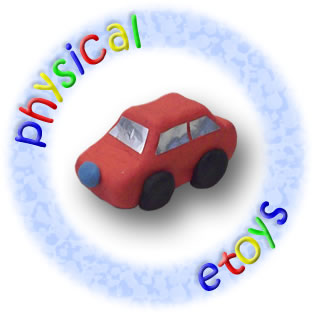
\includegraphics[width=8cm]{physical_etoys_logo.jpg}\\
	\vfill
	%
\includegraphics[width=5cm]{minibot.png}
	\vspace{3em}
	\LARGE{\textbf{\appName et la carte Arduino}}\\[1cm]
	\large{Les premiers pas pour programmer la carte Arduino avec \appName}\\[1cm]
	\vfill
}

\author{
GIRA \\
Version française : Planète Sciences
}

%%%%%%%%%%%%%%%%%%%%%%%%%%%%%%%%%%%%%%%%%%%%%%%%%%%%%%%%%%%%%%%%%%%%%%%%%%%%%%%%%
%%%%%%%%%%%%%%%%%%%%%%%%%%%%%%%%%%%%%%%%%%%%%%%%%%%%%%%%%%%%%%%%%%%%%%%%%%%%%%%%%
\begin{document}

% If a PDF file called 'cover.pdf' exists, use it as cover.
\IfFileExists{cover.pdf}{
\includepdf[pages=-, fitpaper]{cover.pdf}
\thispagestyle{empty}
\cleardoublepage
}

\maketitle

\cleardoublepage
\tableofcontents
\cleardoublepage

En raison de la popularité et des différentes fonctionnalités de la carte
Arduino, nous allons voir dans ce tutoriel comment accéder à certaines d'entre
elles depuis \appName : au programme, des petits scripts simples et une
introduction à l'électronique.

%%%%%%%%%%%%%%%%%%%%%%%%%%%%%%%%%%%%%%%%%%%%%%%%%%%%%%%%%%%%%%%%%%%%%%%%%%%%%%%%%
\section{Installation}

\subsection{Ce qu'il vous faut}

\begin{itemize}
        \item une carte Arduino (nous avons testé avec la Duemilanove),
        \item un cable USB,
        \item le logiciel \appName.
\end{itemize}


\subsection{En option...}

Une LED, un petit bouton poussoir, une carte de prototypage pour faire des
essais de branchements, 3 résistances 10 KOhms et un servo-moteur. Ce matériel
nous permettra de vérifier que la carte fonctionne. 

\subsection{Installation des pilotes}

Lorsque vous connectez la carte Arduino, Windows la détecte et lance la
procédure d'installation de pilote (si c'est la première fois que vous utilisez
une Arduino avec votre ordinateur).

Sous Windows Vista, le pilote devrait être téléchargé et installé
automatiquement.

Sous Windows XP, l'assistant d'ajout de matériel va s'ouvrir :

\begin{itemize}
        %TODO: CQ: Faudrait, pour être parfait, refaire la procédure pour avoir les termes exacts...  
        %D'autre part, les choses sont légèrement différentes avec une 2009 et une UNO (pas le même pilote, donc termes légèrement différents). 
        %Ici, c'est pour une 2009 manifestement.
        \item 

		Sélectionnez l'option \og Non, pas cette fois ci \fg lorsque Windows
		essaie d'effectuer une recherche automatique de pilote. Cliquez sur \og
		Suivant \fg.
        
        \item 

		Sélectionnez \og Installer depuis une liste ou un emplacement
		spécifique (utilisateurs avancés) \fg puis cliquez sur \og Suivant \fg


        \item

		Assurez vous que l'option \og Rechercher le meilleur pilote à cet
		emplacement \fg est sélectionée ; désélectionnez \og Media amovibles
		\fg; sélectionnez \og Inclure cet emplacement \fg et indiquez le chemin
		d'accès du répertoire \code{/FTDI USB Drivers} de l'installation
		Arduino.  si nécessaire, les tout derniers pilotes peuvent être
		téléchargés sur le site de FTDI (cartes Duemillanove, notamment) ou
		bien d'Arduino directement (cartes UNO).  Cliquez sur "suivant".
        
        \item

		L'assistant va rechercher le pilote, puis indiquer qu'un \og
		Convertisseur série USB \fg a été détecté (Duemillanove), ou bien une
		carte Arduino (UNO). Cliquez sur \og Terminer \fg.
        
        \item
		L'assistant d'installation de nouveau matériel est alors relancé
		(Duemillanove). Suivez les même étapes que précédemment. Cette fois-ci,
		un \og Port série USB \fg est détecté et installé.

\end{itemize}

Vous pouvez vérifier que le pilote a été installé en ouvrant le gestionnaire de
périphériques de Windows (onglet "matériel" dans le panneau de contrôle
système).  Dans la catégorie \og Ports \fg, vous devriez voir apparaitre la
carte Arduino sous la forme d'un \og Port série USB \fg (Duemillanove), ou bien
directement avec le nom "Arduino".

%%%%%%%%%%%%%%%%%%%%%%%%%%%%%%%%%%%%%%%%%%%%%%%%%%%%%%%%%%%%%%%%%%%%%%%%%%%%%%%%%
\section{Connecter la carte Arduino à \appName}

Avant tout, il nous faut avoir un objet graphique représentant la carte Arduino
sous \appName.

Pour l'obtenir, cliquez sur l'icône du tiroir \og Accessoires \fg.

\screenshot{01.png}

Le tiroir \og Accessoires \fg contient les objets les plus utilisées. Nous en
apprendrons plus à leur sujet au fur et à mesure. Celui qui nous interesse pour
le moment est le catalogue d'objets. %TODO: à vérifier dans la traduction
francaise d'etoys!

\screenshot{02.png}

Déposer le catalogue d'objet sur le bureau de \appName.

\screenshot{03.png}

Le catalogue est une sorte de boîte contenant tous les objets que l'on peut
utiliser. Ils sont classés par catégories mais vous pouvez les aussi les trier
de manière alphabétique.

Maintenant choisissez la catégorie \og Électronique\fg. Puis glissez/déposez le
symbole de la carte Arduino sur le bureau.

\screenshot{04.png}
  
Maintenant, nous pouvons afficher le visualisateur de la carte en faisant un
\rc sur son image. Ceci affiche une série d'icônes autour de la carte qu'on
appelle le \keyword{halo}. Les différentes icônes permettent de modifier,
supprimer, agrandir ou rétrécir l'objet.

En cliquant sur \icon[\oe il]{eye}, le visualisateur apparait. Le visualisateur
est un panneau qui permet non seulement de voir et modifier les propriétés des
objets, mais aussi de créer des \important{scripts}. Les scripts sont les
petits programmes qui vont animer nos objets (les faire bouger, tourner ou ...
contrôler la carte Arduino).  Les propriétés et les actions sont représentés
par des \important{briques}.

\screenshot{05.png}

Dans la catégorie appelée "connection à la carte arduino" vous pourrez trouver
des informations très utiles pour connecter votre carte Arduino. Pour changer
de catégorie il faut double cliquer sur le petit triangle en haut à gauche du
titre de la catégorie puis choisir la catégorie désirée

\screenshot{06.png}

Nous devons d'abord spécifier quelle carte nous allons utiliser. Dans notre
exemple nous choisirons la carte Duemilanove avec le microcontroleur ATmega328.
Puis il faut définir le port COM par lequel la carte est connectée. Pour le
savoir il suffit de cliquer droit sur "Poste de travail" ou "Ordinateur" (si
vous êtes sur PC Windows) puis "propriétés". Puis dans le disque dur, cliquez
sur"gestionnaire de système" ?

\screenshot{07.png}

Maintenant regardez dans la section "ports" et une fois dedans vous verrez le
numéro du port USB près de l'inscription "port série USB". Dans notre exemple
c'est le port 8.
 
\screenshot{08.png}

Donc la valeur correspondant au port sous squeakbot sera COM 8

\screenshot{09.png}

Maintenant il est important de cliquer sur "connecter". Si nous chargeons cette
commande (en cliquant sur   ), nous connecterons Arduino avec     et la case
indiquant que la carte Arduino est connectée changera sa valeur en "vrai".

\screenshot{10.png}

Si  c'est la première fois que vous essayer de connecter Arduino, une fenêtre
apparaitra vous demandant si vous désirez installer Firmata. Firmata est le
programme contenant le protocole de communication permettant à la carte de
recevoir des commandes. Il faut donc cliquer sur "oui".

\screenshot{11.png}

Une barre de progression vous indiquera où vous en êtes dans l'installation.
 
\screenshot{12.png}

Si tout se passe bien, une légende apparaitra pour indiquer que l'installation
s'est correctement réalisée. Maintenant il faut encore connecter la carte
Arduino (en cliquant sur le point d'exclamation de la case associée). Si la
carte Arduino est connectée, la brique \tile{est connectée} passe à
\tile{vrai}.

\screenshot{13.png}

%%%%%%%%%%%%%%%%%%%%%%%%%%%%%%%%%%%%%%%%%%%%%%%%%%%%%%%%%%%%%%%%%%%%%%%%%%%%%%%%%
\section{Les premiers pas : faire clignoter une LED}

Avant de pouvoir utiliser \appName, il est nécessaire de connecter
physiquement la LED à la carte.  Dans cet exemple, la cathode doit être
reliée à la masse (\code{GND}) et l'anode à la treizième broche (D13).

%TODO/remarque(CQ): est-ce qu'on ferait pas une petite phrase pour dire que:
%- ya déjà une LED sur la carte pour la pin13 (elle est petite, certes, mais déjà présente)
%- pas besoin de mettre une résistance parce que yen a déjà une sur D13, mais dans le cas général, il en faut une
%- comment on identifie anode & cathode ?

\screenshot{14.jpg}

\screenshot{15.png}

Il est désormais possible de commencer avec \appName.

Dans la catégorie \og électronique \fg, sélectionnons une LED, qu'on peut
glisser et déposer dans la fenêtre principale.

\screenshot{16.png}

Une fois que la LED est placée dans la fenêtre principale, cliquons sur sa
broche \code{+} pour faire apparaitre un fil, qu'on peut ensuite relier à une
des broches de l'objet \og Arduino \fg (dans notre cas: la broche D13).

\screenshot{17.png}

Ensuite, allons dans le visualisateur de la LED, pour faire apparaitre ces briques :

\screenshot{18.png}

Créons maintenant un nouveau script pour faire clignoter la LED.

Pour cela, il faut glisser/déposer la brique \tile{script vide} qui se trouve
dans la catégorie \og scripts \fg. Une fois que ceci est fait, on obtient cela
:

\screenshot{19.png}

Ensuite, il faut cliquer sur \icon[boite à outil]{toolbox} et choisir une
brique \testtile{}.

Cette brique signifie que le script va faire quelque chose selon une condition
donnée (dans ce cas, la valeur de la LED).%TODO:, représentative de son état).

Pour ceux qui ont déjà quelques notions de programmation, cette brique est une
\og structure conditionnelle \fg (ou structure \og IF \fg).

\screenshot{20.png}

Afin de définir notre condition, il faut attraper la brique \tile{led value} et
venir la déposer à côté de \testtile{Test} (attention, il ne faut pas prendre
la brique par la \icon{greenarrow} flêche verte puisque nous voulons
\important{utiliser} la valeur de la LED, et non lui \important{assigner} une
valeur).

\screenshot{21.png}

Maintenant, nous devons décider de ce que le script va faire lorsque la LED est
allumée. Très logiquement, nous voulons ... l 'éteindre. Donc cette fois-ci, il
faut \important{assigner} la valeur \code{Faux} à la LED. Il faut donc prendre
la brique \tile{led value} par la \icon{greenarrow} flêche verte.

\screenshot{22.png}

\screenshot{22b.png}

Maintenant, nous allons faire la même chose avec une petite différence : quand
la LED est éteinte, \appName  la fera s'allumer.  Nous devons donc faire
glisser la brique \tile{led value} avec sa \icon{greenarrow} flêche en face du
\testtile{Non} de la brique \testtile{}, en s'assurant que sa valeur est
\tile{vrai}.

\screenshot{23.png}

Pour conclure, nous pouvons démarrer le script en cliquant sur
\icon[horloge]{startscript}.

\screenshot{24.png}

Si tout fonctionne correctement, la LED va clignoter.

%%%%%%%%%%%%%%%%%%%%%%%%%%%%%%%%%%%%%%%%%%%%%%%%%%%%%%%%%%%%%%%%%%%%%%%%%%%%%%%%%
\section{Allumer une LED en appuyant sur un bouton}


Dans la catégorie \og Électronique \fg du catalogue d'objet, attrapons le
\important{Bouton poussoir}, pour le connecter ensuite à la deuxième broche de
la carte Arduino :

\screenshot{25.png}


Il vaut mieux arrêter le script précédent (en cliquant sur
\icon[Stop]{pausescript}) pour cette partie. Par contre, gardons la LED
branchée sur la broche 13.

Connectons le bouton (avec la résistance sur la carte de prototypage) comme
ceci :

\screenshot{26.png}

\screenshot{27.png}

Maintenant, ouvrons le visualiseur du bouton poussoir et créons un nouveau
script.

\screenshot{28.png}

Ajoutons ensuite une brique \testtile{} afin de savoir quand le bouton est
pressé. Nous devons faire glisser la brique avec son nom car ce n'est pas une
instruction. Nous voulons juste connaitre sa valeur.

\screenshot{29.png}

Quand le bouton est appuyé nous voulons assigner à la LED la valeur
\code{vrai}, dans l'autre cas, nous lui assignons la valeur faux. N'oubliez pas
faire glisser la brique avec sa \icon{greenarrow} flêche. Pour conclure,
démarrons le script en cliquant sur \icon[horloge]{startscript}.

\screenshot{30.png}

Si tout fonctionne correctement, quand on appuie sur le bouton, la LED clignote.

%%%%%%%%%%%%%%%%%%%%%%%%%%%%%%%%%%%%%%%%%%%%%%%%%%%%%%%%%%%%%%%%%%%%%%%%%%%%%%%%%
\section{Utiliser une photo-résistance}

Tant que la carte Arduino est connectée, nous allons ajouter une
photorésistance (qui est dans la catégorie \og Électronique \fg) à la seconde
broche des entrées analogiques.

\screenshot{31.png}

Une fois branché, le montage ressemble à celà :

\screenshot{32.png}

\screenshot{33.png}

Maintenant, ouvrons le visualiseur de la photorésistance et creons un nouveau
script. Ouvrons le catalogue d'objet et faisons glisser un rectangle à partir
de la catégorie des objets de base. Ensuite ouvrons le visualiseur du rectangle
afin de faire glisser (avec sa flêche) la tuile luminosité dans le script de la
photorésistance. Maintenant, ouvrons le visualiseur de la photorésistance pour
remplacer la valeur de la luminosité du rectangle (\tile{100}) par la brique
\tile{light value de la  photorésistance}(sans la flêche, car nous voulons
juste lire la valeur).

\screenshot{34.png}

Pour finir, nous pouvons exécuter le script pour voir comment les rectangle
font varier leur luminosité en fonction de la lumière ambiante.

%%%%%%%%%%%%%%%%%%%%%%%%%%%%%%%%%%%%%%%%%%%%%%%%%%%%%%%%%%%%%%%%%%%%%%%%%%%%%%%%%
\section{Faire tourner un servo-moteur avec un rectangle}

Avec la carte Arduino toujours connectée, branchons un servo-moteur (lui-aussi
dans la catégorie \og Électronique \fg) sur la septième broche.

\screenshot{35.png}

Sur la carte réelle, ça doit ressembler à ça :

\screenshot{36.png}

Afin de gagner du temps, nous pouvons réutiliser le rectangle créé dans le
dernier exercice. Ouvrons son halo, et utilisons \icon[Mise à l'échelle]{scale}
pour changer sa taille.

\screenshot{37.png}

Maintenant, il faut ouvrir le visualisateur du servo-moteur et créer un nouveau
script avec la brique \tile{servo's degrees}. Nous voulons modifier cette
valeur, donc une fois encore, c'est un assignement et nous devons attraper la
brique par sa \icon{greenarrow} flêche.

\screenshot{38.png}

Ensuite, il faut ouvrir le visualisateur du rectangle, et dans la catégorie
\code{Briques de base}, prendre la brique \tile{cap}.

Nous pouvons démarrer le script.

\screenshot{39.png}

Pendant que le script \og tourne \fg, ouvrons le halo du rectangle. Pour finir,
faisons glisser \icon[Faire tourner]{rotate} pour faire tourner le rectangle.

\screenshot{40.png}

Si tout s'est bien passé, le servo-moteur devrait tourner en même temps que le
rectangle.

%%%%%%%%%%%%%%%%%%%%%%%%%%%%%%%%%%%%%%%%%%%%%%%%%%%%%%%%%%%%%%%%%%%%%%%%%%%%%%%%%
\section{Conclusion}

Voilà, c'est tout ce dont vous avez besoin pour commencer à utiliser la carte
Arduino. Les possibilités d'interaction entre l'ordinateur, Arduino et les
autres composants électroniques que fournit \appName sont très nombreuses : nous
vous encourageons à découvrir les autres fonctions et composants en explorant
le reste de l'environnement Squeak (et pour celà, rien de tel que tester,
jouer, toucher et même en casser si besoin !).

Amusez-vous bien !

%%%%%%%%%%%%%%%%%%%%%%%%%%%%%%%%%%%%%%%%%%%%%%%%%%%%%%%%%%%%%%%%%%%%%%%%%%%%%%%%%
%%%%%%%%%%%%%%%%%%%%%%%%%%%%%%%%%%%%%%%%%%%%%%%%%%%%%%%%%%%%%%%%%%%%%%%%%%%%%%%%%
\printglossaries

%%%%%%%%%%%%%%%%%%%%%%%%%%%%%%%%%%%%%%%%%%%%%%%%%%%%%%%%%%%%%%%%%%%%%%%%%%%%%%%%%%%%%%%%%%%%%%%%%%%%%%%
\clearpage
\thispagestyle{empty}
~
\vfill
\begin{center}
        GIRA 2011\\
        Planète Sciences 2011 pour la version française.
        Cette documentation est diffusée sous les termes de la licence Creative Commons Paternité-Partage à l'identique.\\
        \vspace{2cm}
        
\includegraphics[scale=0.5]{logo_cc.png}
\end{center}

\vfill

\begin{center}
        Les sources LaTeX originales de ce guide peuvent être téléchargées sur GitHub.
        \url{http://github.com/GIRA/Physical-Etoys}
\end{center}

\vfill

\end{document}
